\subsection{Введение}

Компьютеры делятся на \textbf{цифровые вычислительные машины (ЦВМ)} и \textbf{аналоговые вычислительные машины (АВМ)}.

ЦВМ работают с числами, которые подаются на вход электрически или механически. Можно рассматривать как структуру из логических вычислительных блоков.

АВМ работают с непрерывными (аналоговыми) сигналами. Используются в системах автоматического управления. Можно рассматривать как структуру из аналоговых вычислительных блоков, выполняющих какую"=то конкретную математическую операцию. В дальнейшем мы будем рассматривать только ЦВМ.

\textbf{Операционная система (ОС)} "--- программа, которая позволяет взаимодействовать с компьютером и периферийными устройствами.

Организация вычислений стала основным толчком в становлении ОС, потому что на заре компьютерной эры время имело ценность для решения расчётных задач. Прародителем современных ОС можно считать программы для одновременной или квазиодновременной работы нескольких пользователей за одной машиной. Они работали следующим образом. Так как процессор работает с некоторой частотой, задаваемой тактовым генератором, решено было отводить часть тактов на одну задачу, а часть на другую. Т.е. применяются квазипараллельные вычисления (в каждый момент времени процессор занят одной задачей, но эти задачи постоянно меняются).

Существовало несколько подходов разделения времени:
\begin{enumerate}
    \item \textbf{Кооперативная многозадачность} "--- время распределяется произвольно.
    \item \textbf{Вытесняющая многозадачность} "--- специальная программа"=планировщик принудительно ставит и снимает задачи по заданному алгоритму планирования (карусель/приоритеты). При этом часть процессорного времени уходит на планирование.
\end{enumerate}

Впоследствии второй подход победил.

Одной из задач планировщика являлось распределение памяти. В связи с этим появилось понятие процесса.

\textbf{Процесс} "--- программа в процессе своего выполнения вместе с некоторыми дополнительными параметрами, такими как отведённая ему память, состояние регистров процессора и т. д.

Требования к информационным системам обусловили требование известного времени работы программы, что привело к появлению \textbf{ОС реального времени}. Напротив "--- \textbf{ОС универсальные}, к ним относятся практически все популярные ОС.

Операционные системы также делятся на \textbf{однопользовательские} и \textbf{многопользовательские ОС}. Введение абстракции пользователя позволило ввести понятие сервиса, из которых состоит сама система.

\textbf{Сервис} "--- подпроцесс, работающий самостоятельно и изолированный от других.

\subsection{Персональные компьютеры}

Миниатюризация электроники привела к появлению машин, имеющих значительно меньшие размеры. Некоторые компании сделали ставку на настольный вариант компьютера.

Коммерческий успех сопутствовал первому ПК "--- \textbf{Apple}.

IBM в ответ создала \textbf{IBM PC}, который имел уже открытую архитектуру, что привело к массе  IBM"=совместимых периферийных устройств и программного обеспечения. Из"=за этого IBM стала одной из ведущих компаний на этом рынке.

Билл Гейтс путем своих связей добился, что на IBM PC будет предустановлена его система на основе DOS. В связи с развитием информационных систем для разных задач на этот ПК возрос спрос, что привело к большому количеству программного обеспечения для DOS.

Появился спрос на графический интерфейс пользователя. Незадолго до выхода ОС с графическим интерфейсом, созданной IBM, Microsoft выпускает недоделанную Windows 95, в которой появляются системные вызовы для работы с графикой.

Таким образом, путь ПК (IBM, Apple) разошелся с остальными компьютерами.

Затем последовали Windows 98, Windows 2000. Параллельно с Windows 95 шла разработка Windows New Technologies "--- система, написанная с нуля.

\subsection{История Unix}

В 1970 г. сотрудники AT\&T Кен Томпсон, Деннис Ритчи и Брайан Керниган разрабатывали систему Multics по заказу министерства обороны США. В свободное время на Ассемблере они написали ОС, ставшую прототипом \textbf{Unix}. Она была быстро переписана на язык C, автором которого был Ритчи. Таким образом, Unix стала первой ОС, написанной на языке высокого уровня, что сделало её переносимой на разные аппараты, так как переписывались лишь драйверы.

Unix быстро стала популярной в учебных заведениях, где её начали изучать. Контора, сотрудниками которой была разработана Unix, зарегистрировала товарный знак UNIX\textregistered\ и сделала её платной. По их задумке студенты, изучавшие Unix, не смогут отказаться от этой ОС и будут вынуждены платить за неё. Крупные игроки залицензировали свои Unix: IBM "--- AIX, Sun Microsystems "--- Solaris. Но студенты и преподаватели переписали код системы и сделали свободно распространяемую версию.

Эндрю Танненбаум написал \textbf{Minix}, построенную на концепции микроядра и получившую распространение на ПК.

Линус Торвальдс заменил в Minix микроядро на монолитное и сделал модифицированную версию "--- \textbf{Linux}, которую опубликовал в интернете. В результате спора с Танненбаумом  Linux остался обозначением для ядра, а не для полноценной ОС.

FreeBSD "--- свободная версия Unix, написанная и спроектированная лучше, чем Linux.

QNX (Quick Unix) "--- коммерческая ОС реального времени с микроядерной архитектурой.

Linux "--- это только ядро, мы же пользуемся \textit{дистрибутивами} Linux. Дистрибутив включает в себя ядро, установщик, пакетный менеджер и набор прикладных программ.

\begin{figure}[H]
	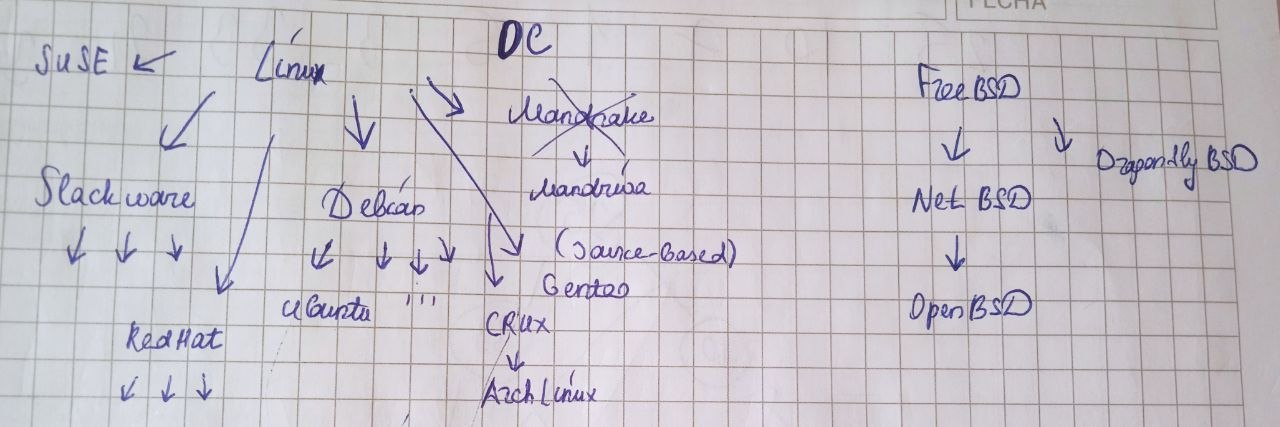
\includegraphics[scale=0.4]{images/linux_distributions.jpg}
	\centering
	\caption{Схема дистрибутивов Linux и FreeBSD}
\end{figure}

Linux From Scratch (LFS) "--- проект, позволяющий создать собственный дистрибутив.

Linux Standard Base (LSB) "--- стандарт, регламентирующий поведение дистрибутива Linux.

Single Unix Specification (SUS) "--- стандарт для Unix.

Изначально Unix предназначался для работы в интернете и традиционно использовался для серверов и сетей.

\subsection{Компьютерные сети}

Изначально владельцы компьютеров (крупного железа) имели свои сети. Internet связал разнородные протоколы, и де"=факто закрепился принцип пакетной передачи данных.

Основной задачей интернета является коммутация каналов/коммутация пакетов.

\textbf{Протокол} "--- соглашение по передаче"=обработке данных. Интернет представляет из себя стек протоколов, причем идея этой архитектуры в том, что работа протокола на каждом уровне не зависит от работы протоколов на более низких уровнях (каждый уровень стека "--- отдельный уровень абстракции).

\begin{figure}[H]
	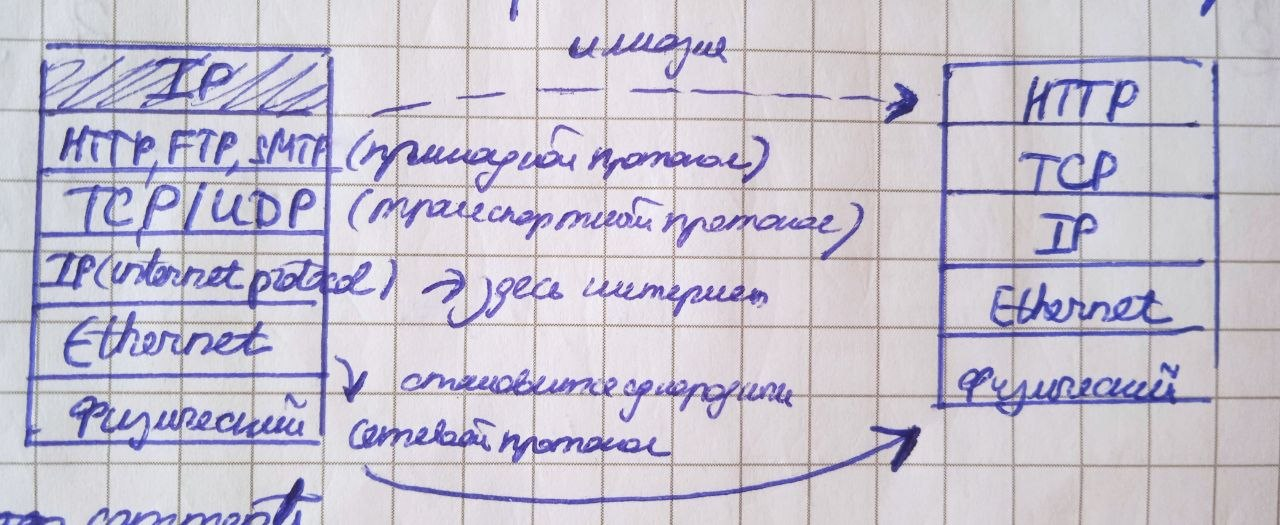
\includegraphics[scale=0.4]{images/protocols.jpg}
	\centering
	\caption{Стек протоколов}
\end{figure}

RFC (requests for comments) "--- серия документов, описывающая все аспекты сетевого взаимодействия интернета.

\subsection{Уровни операционной системы}

\begin{enumerate}
	\item Kernel "--- ядро, внутренний уровень;
	\item Shell "--- оболочка, внешний уровень.
\end{enumerate}

X Window System "--- графическая оболочка.

XLog "--- окно входа X Server.

\subsection{Системные вызовы}

Аналог команды cp с помощью высокоуровневых функций работы с файлами:

\begin{minted}{c}
FILE* fv = fopen("from.txt", "r");
FILE* tv = fopen("to.txt", "w");
while ((c = getc(fv)) != EOF) putc(c, tv);
fclose(fv);
fclose(tv);
\end{minted}

Системные вызовы для работы с файлами:

\begin{itemize}
\item Создание файла:
\begin{minted}{c}
creat("file.txt", 0642);
\end{minted}

\item Сброс прав по умолчанию:
\begin{minted}{c}
umask(0);
\end{minted}

\item Создание файла и запись в него:
\begin{minted}{c}
char buf[10];
umask(0);
int fd = creat("file.txt", 0642);
write(fd, buf, sizeof(buf));
close(fd);
\end{minted}

\item Открытие файла (старый способ):
\begin{minted}{c}
int mode = 1; // 0 - r, 1 - w, 2 - rw
open("file.txt", mode);
\end{minted}

\item Открытие файла (новый способ):

Применяются флаги, их можно комбинировать через побитовое или (|).
\begin{enumerate}
    \item \texttt{O\_CREAT} "--- создать файл, если его не существует;
    \item \texttt{O\_RDONLY} "--- открыть только для чтения;
    \item \texttt{O\_WRONLY} "--- открыть только на запись;
    \item \texttt{O\_RDWR} "--- открыть на чтение и запись;
    \item \texttt{O\_APPEND} "--- запись в конец файла;
    \item \texttt{O\_NDELAY} "--- не блокировать при открытии;
    \item \texttt{O\_TRUNC} "--- сократить размер файла до нуля.
    \item \texttt{O\_EXCL} "--- ошибка, если файл существует (в сочетании с \texttt{O\_CREAT}).
\end{enumerate}

\begin{minted}{c}
int fd = open("from.txt", O_RDONLY);
int to = open("to.txt", O_WRONLY | O_CREAT);
char buf[10];
while ((n = read(fd, buf, sizeof(buf))) > 0) {
	write(to, buf, n);
}
\end{minted}

\item Перенос указателя:

Сдвинуть указатель файлового дескриптора \texttt{fd} на 3 байта вправо с начала:
\begin{minted}{c}
lseek(fd, 3, 0);
\end{minted}

\item Создание жёсткой ссылки (hard link):

\begin{minted}{c}
link("oldfile.txt", "newfile.txt");
\end{minted}

\item Удаление ссылки (файл удалится, когда удалится последняя ссылка, указывающая на него):

\begin{minted}{c}
unlink("file.txt");
\end{minted}

\item Создание символической ссылки (файл специального типа, как ярлык):

\begin{minted}{c}
symlink("oldfile.txt", "newfile.txt");
\end{minted}

\end{itemize}

Стандартные потоки: $0$ "--- \texttt{stdin}, $1$ "--- \texttt{stdout}, $2$ "--- \texttt{stderr}.
